\section{Explaining Goodhart's Law in Reinforcement Learning}\label{sec:explain_goodhart}

\begin{figure}[t]
    % \vspace{-3mm}
    \centering
    \begin{subfigure}[b]{0.33\textwidth}
        \centering
        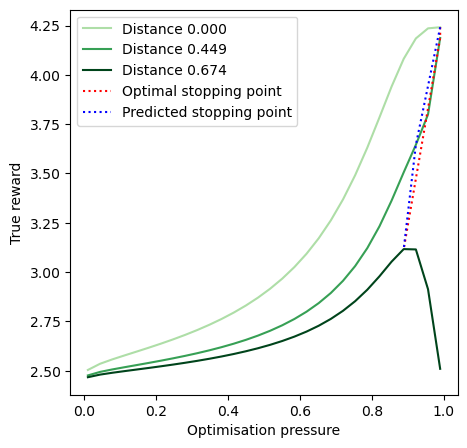
\includegraphics[width=1\textwidth]{example/example_mce_plot_1.png}
        \caption{Goodharting behavior in $\mathcal{M}_{2, 2}$ over three reward functions. Our method is able to predict the optimal stopping time (in blue).}
        \label{subfig:2-2-mce}
    \end{subfigure}
    \hfill
    \begin{subfigure}[b]{0.63\textwidth}
        \centering
        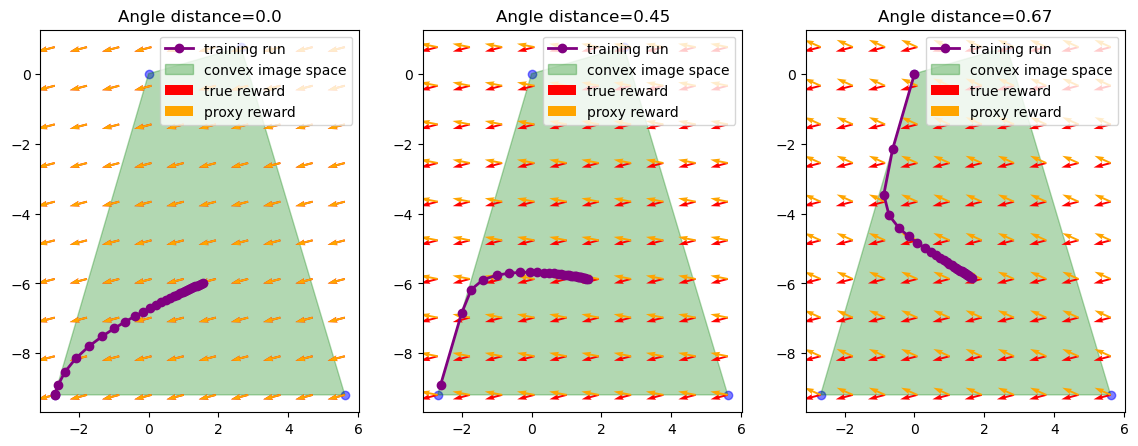
\includegraphics[width=1\textwidth]{example/example_mce_plot_trajectory.png}
        \caption{Training runs for each of the reward functions embedded in the state-action occupancy measure space. Even though the full frequency space is {$|S||A| = 4$-dimensional}, the image of the policy space occupies only a {$|S|(|A| - 1) = 2$-dimensional} linear subspace. Goodharting occurs when the cosine distance between rewards passes the critical threshold and the policy snaps to a different endpoint.}
        \label{subfig:2-2-mce-image}
    \end{subfigure}
    \caption{Visualisation of Goodhart's law in case of $\mathcal{M}_{2, 2}$.}
    \label{fig:2-2-mce-example}
\end{figure}

In this section, we provide an intuitive, mechanistic account of \emph{why} Goodharting happens in MDPs, that explains some of the results in Section~\ref{sec:quantifying_goodharting}. An extended discussion is also given in Appendix~\ref{appendix:extra_explanation}.

First, recall that $\J_\R(\policy) = \occmeas{\policy} \cdot \R$, where $\occmeas{\policy}$ is the occupancy measure of $\pi$. Recall also that $\Polytope$ is a convex polytope.
Therefore, the problem of finding an optimal policy can be viewed as maximising a linear function $\R$ within a convex polytope $\Polytope$, which is a linear programming problem.


\emph{Steepest ascent} is the process that changes $\vec{\occmeaselem}$ in the direction that most rapidly increases $\vec{\occmeaselem}\cdot \R$
\charlie{This feels informal. What is ``most rapidly increases''? The direction which most rapidly increases reward is the direction of the reward.}\oliver{Not when you're on the boundary. This is correct.}
(for a formal definition, see \cite{chang_steepest_1989} or \cite{denel_steepest_1981}). The path of steepest ascent forms a piecewise linear curve whose linear segments lie on the boundary of $\Polytope$ (except the first segment, which may lie in the interior). Due to its similarity to gradient-based optimisation methods, we expect most policy optimisation algorithms to follow a path that roughly approximates steepest ascent. \charlie{`we should expect' is a red-flag. We either need to justify this claim with intuition or use weaker language.}
Steepest ascent also has the following property:

\begin{proposition}[Concavity of Steepest Ascent]\label{prop:concave_proof}
If $\TangentVec_i := \frac{\occmeaselem_{i+1}-\occmeaselem_i}{||\occmeaselem_{i+1}-\occmeaselem_i||}$ for $\occmeaselem_i$ produced by steepest ascent on reward vector $\R$, then $\TangentVec_i \cdot \R$ is decreasing. 
\end{proposition}
\charlie{The title of this proposition uses the word `concave' but it's unclear to me what this refers to. I see now there is a line that is commented out, but still not sure what it means or what value it's adding.}

We can now explain Goodhart's law in MDPs.
Assume we have a true reward $\TrueR$ and a proxy reward $\ProxR$, that we optimise $\ProxR$ through steepest ascent, and that this produces a sequence of occupancy measures $\{\eta_i\}$.
Recall that this sequence forms a piecewise linear path along the boundary of a convex polytope $\Omega$, and that $\J_{\TrueR}$ and $\J_{\ProxR}$ correspond to linear functions on $\Omega$ (whose directions of steepest ascent are given by $\QProj_\T \TrueR$ and $\QProj_\T \ProxR$).
First, if the angle between $\QProj_\T \TrueR$ and $\QProj_\T \ProxR$ is less than $\pi/2$, and the initial policy $\eta_0$ lies in the interior of $\Omega$, then it is guaranteed that $\eta \cdot \TrueR$ will increase along the first segment of $\{\eta_i\}$.
However, when $\{\eta_i\}$ reaches the boundary of $\Omega$, steepest ascent continues in the direction of the projection of $\QProj_\T \ProxR$ onto this boundary. If this projection is far enough from $\TrueR$, optimising in the direction of $\QProj_\T \ProxR$ would lead to a decrease in $\J_{\TrueR}$ (c.f.\ Figure~\ref{subfig:2-2-mce-image}). \emph{This corresponds to Goodharting}.\oliver{someone else look over please}


$\TrueR$ may continue to increase, even after another boundary region has been hit.
However, each time $\{\eta_i\}$ hits a new boundary, it changes direction, and there is a risk that $\eta \cdot \TrueR$ will decrease.
In general, this is \emph{more} likely if the angle between that boundary and $\{\eta_i\}$ is close to $\pi/2$, and \emph{less} likely if the angle between $\QProj_\T\TrueR$ and $\QProj_\T\ProxR$ is small. This explains why Goodharting is less likely when the angle between $\QProj_\T\TrueR$ and $\QProj_\T\ProxR$ is small. 
%
Next, note that Proposition~\ref{prop:concave_proof} implies that the angle between $\{\eta_i\}$ and the boundary of $\Omega$ will increase over time along $\{\eta_i\}$. This explains why Goodharting becomes more likely when more optimisation pressure is applied.

Let us consider an example to make our explanation of Goodhart's law more intuitive.
Let $\mathcal{M}_{2, 2}$ be an MDP with 2 states and 2 actions, and let $R_0, R_1, R_2$ be three reward functions in $\mathcal{M}_{2, 2}$.
The full specifications for $\mathcal{M}_{2, 2}$ and $R_0, R_1, R_2$ are given in Appendix~\ref{appendix:simple_goodharting_example}.
We will refer to $R_0$ as the \emph{true reward}.
The angle between $R_0$ and $R_1$ is larger than the angle between $R_0$ and $R_2$.
Using Maximal Causal Entropy, we can train a policy over each of the reward functions, using varying degrees of optimisation pressure, and record the performance of the resulting policy with respect to the \emph{true} reward.
Zero optimisation pressure results in the uniformly random policy, and maximal optimisation pressure results in the optimal policy for the given proxy (see ~\Cref{subfig:2-2-mce}).
As we can see, we get Goodharting for $R_2$ -- increasing $R_2$ initially increases $R_0$, but there is a critical point after which further optimisation leads to worse performance under $R_0$.


To understand what is happening, we embed the policies produced during each training run in $\Omega$, together with the projections of $R_0, R_1, R_2$ (see ~\Cref{subfig:2-2-mce-image}). We can now see that Goodharting must occur precisely when the angle between the true reward and the proxy reward passes the critical threshold, such that the training run deflects upon stumbling on the border of $\Omega$, and the optimal deterministic policy changes from the lower-left to the upper-left corner.
\emph{This is the underlying mechanism that produces Goodhart behaviour in reinforcement learning!}

We thus have an explanation for why the Goodhart curves are so common.
Moreover, this insight also explains why Goodharting does not always happen and why a smaller distance between the true reward and the proxy reward is associated with less Goodharting. We can also see that Goodharting will be more likely when the angle between $\{\eta_i\}$ and the boundary of $\Omega$ is close to $\pi/2$ -- this is why Proposition~\ref{prop:concave_proof} implies that Goodharting becomes more likely with more optimisation pressure.

